
\renewcommand{\EntradaBibtex}{MarcoNuno_Revista_2018_08_00}
\begin{frame}{\citetitle{\EntradaBibtex} \footnotemark[1] (1)}


%\begin{frame}{\citetitle{MarcoNuno_Revista_2018_08_00} \footnotemark (1)}
%\begin{block}{Aplicación para Enseñanza de Robótica utilizando Realidad Aumentada \footnotemark (1)} 
\begin{columns}
\begin{column}{0.5\textwidth}
Componentes:
		\begin{itemize}
		\item Un sistema (Arduino) que genera los movimientos del brazo robot incluye un transmisor Bluetooth
		\item Una aplicación móvil que visualizar un transportador virtual encima de una articulación robótica con el ángulo en tiempo real
		\end{itemize}
\end{column}
\begin{column}{0.5\textwidth}  
    \begin{center}
     %%%%% this is a minipage, so \textwidth is already adjusted to the size of the column
     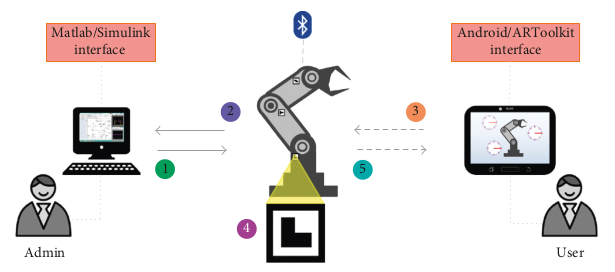
\includegraphics[width=0.9\textwidth]{Figs/SistemaAR_Maestria1}
     \end{center}
\end{column}
\end{columns}
%\end{block} 
\footnotetext[1]{\fullcite{\EntradaBibtex}}

\end{frame}

\begin{frame}{\citetitle{\EntradaBibtex} (2)}
%\begin{block}{Aplicación para Enseñanza de Robótica utilizando Realidad Aumentada (2)} 
\begin{columns}
\begin{column}{0.5\textwidth}
Funcionamiento de la aplicación:
		\begin{itemize}
		\item Se emplea un marcador ARUCO para determinar de que articulación se trata
		\item Mediante comandos Bluetooth se obtiene el ángulo
		\end{itemize}
\begin{center}
     %%%%% this is a minipage, so \textwidth is already adjusted to the size of the column
     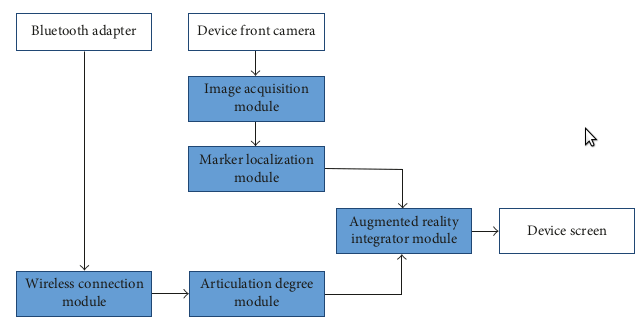
\includegraphics[width=0.79\textwidth]{Figs/SistemaAR_Maestria2}
     \end{center}
\end{column}
\begin{column}{0.5\textwidth}  
    \begin{center}
     %%%%% this is a minipage, so \textwidth is already adjusted to the size of the column
     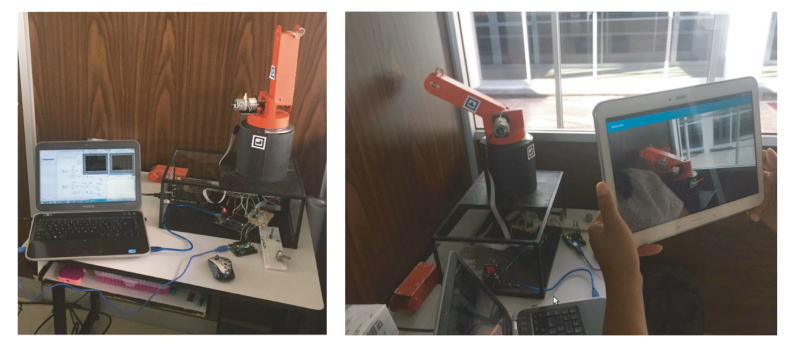
\includegraphics[width=0.79\textwidth]{Figs/SistemaAR_Maestria3}
     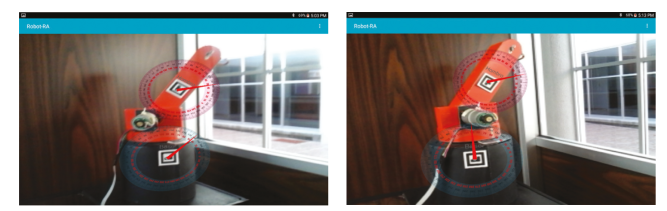
\includegraphics[width=0.79\textwidth]{Figs/SistemaAR_Maestria4}
     \end{center}
\end{column}
\end{columns}
%\end{block} 
\end{frame}


